\documentclass[11pt,oneside]{book}

% ---------- Packages ----------
\usepackage[utf8]{inputenc}
\usepackage[T1]{fontenc}
\usepackage{graphicx}
\usepackage[margin=1in]{geometry}
\usepackage{xcolor}
\usepackage{listings}
\usepackage{enumitem}
\usepackage{hyperref}
\usepackage{fancyhdr}
\usepackage{titlesec}
\usepackage{tabularx}
\usepackage{booktabs}
\usepackage{longtable}
\usepackage{array}
\usepackage{amssymb}
\usepackage{caption}
\usepackage{pifont} % for \ding checkmark symbols
\usepackage{float}  % for [H] "exactly here" figure placement, so figures stay with their topic

% ---------- Colors ----------
% Per author request: the document body (titles, headings, links) is black.
% Only RTL/.sv file paths get a distinguishing style so they still stand out
% as "code", but without using a loud color like blue/green.
\definecolor{rtlgray}{gray}{0.35}      % dark gray "code" tone for RTL paths (reads as near-black)

% ---------- Custom command for RTL file paths ----------
% Distinguishes RTL paths as "code" via italic monospace in a muted dark-gray
% tone, instead of a colored highlight box. A background \colorbox cannot
% break across lines, which overflowed long paths inside table cells, so
% plain (unboxed) styled text is used here -- it wraps normally via \url,
% which breaks properly at "/" and "_". soul.sty is not available in this build.
\urlstyle{tt}
\newcommand{\rtl}[1]{\textit{\textcolor{rtlgray}{\url{#1}}}}

% A block for a list of RTL references (also highlighted, boxed)
\newenvironment{rtlrefs}{%
  \begin{quote}
  \noindent\textbf{RTL References}\par
  \vspace{2pt}
  \begin{itemize}[leftmargin=*,itemsep=1pt,topsep=2pt]
}{%
  \end{itemize}
  \end{quote}
}
\newcommand{\rtlitem}[1]{\item \rtl{#1}}

% ---------- Section numbering depth ----------
\setcounter{secnumdepth}{3}
\setcounter{tocdepth}{2}

% ---------- Headers/Footers ----------
\setlength{\headheight}{14pt}
\pagestyle{fancy}
\fancyhf{}
\fancyhead[LE,RO]{\thepage}
\fancyhead[RE]{\nouppercase{\leftmark}}
\fancyhead[LO]{\nouppercase{\rightmark}}
\renewcommand{\headrulewidth}{0.4pt}

% ---------- Chapter/Section title styling ----------
\titleformat{\chapter}[display]
  {\normalfont\huge\bfseries}
  {\chaptertitlename\ \thechapter}{20pt}{\Huge}
\titleformat{\section}
  {\normalfont\Large\bfseries}{\thesection}{1em}{}
\titleformat{\subsection}
  {\normalfont\large\bfseries}{\thesubsection}{1em}{}

% ---------- Graphics path ----------
\graphicspath{{figures/}}

% ---------- Hyperref setup ----------
\hypersetup{
  colorlinks=true,
  linkcolor=black,
  urlcolor=black,
  citecolor=black,
  pdftitle={Understanding the Sargantana Microarchitecture},
  pdfauthor={Muhammad Waleed Akram}
}

\title{Understanding the Sargantana Microarchitecture}
\author{Muhammad Waleed Akram}
\date{}

\begin{document}

% ================= TITLE PAGE =================
\begin{titlepage}
\centering
\vspace*{1.5cm}

{\Huge\bfseries Understanding the\\[4pt] Sargantana Microarchitecture\par}
\vspace{0.6cm}
{\Large An RTL-Oriented Study of the Sargantana RISC-V Processor\par}

\vspace{2cm}

\begin{minipage}{0.42\textwidth}
  \centering
  
\includegraphics[width=0.55\textwidth]{sargantana_logo.png}
\end{minipage}%
\begin{minipage}{0.42\textwidth}
  \centering
  
\includegraphics[width=0.5\textwidth]{riscv_logo.png}
\end{minipage}

\vspace{2cm}

{\Large\bfseries Author\par}
{\Large Muhammad Waleed Akram\par}

\vspace{1.5cm}

{\large Repository: \url{https://github.com/bsc-loca/sargantana}\par}

\vfill

{\large \today\par}

\end{titlepage}

\frontmatter
\tableofcontents

\mainmatter

\chapter{Introduction}

\section{About Sargantana}

Sargantana is an open-source, Linux-capable, high-performance RISC-V processor developed
by the Barcelona Supercomputing Center (BSC). It is designed as an out-of-order superscalar
processor capable of executing multiple instructions simultaneously while maintaining precise
architectural state. Unlike simple in-order RISC-V processors commonly used for educational
purposes, Sargantana incorporates modern microarchitectural techniques such as speculative
execution, branch prediction, register renaming, out-of-order execution, and in-order instruction
retirement.

\section{Key Features}

Some of the primary architectural features of the Sargantana processor include:

\begin{itemize}
  \item Open-source RISC-V implementation.
  \item Linux-capable processor architecture.
  \item Out-of-order instruction execution.
  \item Superscalar instruction issue.
  \item Multi-stage pipelined datapath.
  \item Dynamic branch prediction.
  \item Speculative instruction execution.
  \item Register renaming using physical registers.
  \item In-order instruction commitment.
  \item Modular RTL organization.
  \item Extensive architectural documentation and design specifications.
\end{itemize}

The processor serves both as a research platform for computer architecture and as a foundation
for exploring advanced hardware features within the RISC-V ecosystem. Owing to its modular
RTL implementation and comprehensive documentation, Sargantana is well suited for
architectural experimentation and ISA extension development.

\section{Objectives of this Study}

The primary objective of this document is to develop a comprehensive understanding of the
Sargantana processor architecture through a systematic study of its RTL implementation and
accompanying documentation. The specific objectives include:

\begin{itemize}
  \item Study the overall Sargantana microarchitecture.
  \item Understand the functionality of each pipeline stage.
  \item Analyze the interaction between the datapath and control logic.
  \item Examine the major RTL modules and their hierarchy.
  \item Relate architectural concepts to their corresponding RTL implementation.
  \item Identify the processor components involved in instruction fetch, execution, and
        retirement.
  \item Understand the processor's recovery and exception handling mechanisms.
  \item Identify potential integration points for the RISC-V Control-Flow Integrity extensions.
\end{itemize}

\section{Repository Organization}

\begin{longtable}{@{}p{0.44\textwidth}p{0.51\textwidth}@{}}
\toprule
\textbf{Directory / File} & \textbf{Description} \\
\midrule
\endhead
\rtldir{rtl/} & Core RTL implementation \\
\rtl{rtl/top\_drac.sv} & Top-level module instantiating datapath, CSR, MMU, HPM \\
\rtldir{rtl/datapath/} & Pipeline stages and execution units \\
\rtl{rtl/datapath/rtl/datapath.sv} & Top-level datapath implementation \\
\rtldir{rtl/datapath/rtl/if\_stage\_1/} & Instruction fetch + branch prediction \\
\rtldir{rtl/datapath/rtl/if\_stage\_2/} & Fetch buffer \\
\rtldir{rtl/datapath/rtl/id\_stage/} & Instruction decode \\
\rtldir{rtl/datapath/rtl/ir\_stage/} & Instruction rename (register renaming, free list) \\
\rtldir{rtl/datapath/rtl/rr\_stage/} & Register read \\
\rtldir{rtl/datapath/rtl/exe\_stage/} & Execution with ALU, FPU, SIMD, load/store/div units \\
\rtldir{rtl/datapath/rtl/wb\_stage/} & Write-back and graduation \\
\rtldir{rtl/control\_unit/} & Control logic \\
\rtl{rtl/control\_unit/rtl/control\_unit.sv} & Top-level control unit module \\
\rtldir{rtl/csr/} & Control/Status Registers and HPM counters (submodule) $\rightarrow$ empty \\
\rtldir{rtl/mmu/} & Memory Management Unit (submodule) $\rightarrow$ empty \\
\rtldir{rtl/common\_cells/} & PULP platform utilities (lzc, fifo, arbiter, etc.) $\rightarrow$ empty \\
\rtldir{doc/} & Documentation \\
\rtldir{doc/specifications/} & Detailed module specifications (LaTeX) \\
\rtl{doc/riscv-spec.pdf} & RISC-V ISA specification \\
\rtl{doc/riscv-privileged.pdf} & RISC-V privileged specification \\
\rtl{doc/sargantana\_pipeline.svg} & Pipeline diagram \\
\rtldir{scripts/} & CI and verification utilities \\
\rtl{scripts/veri\_lint.sh} & Verilator linting \\
\rtl{scripts/questa\_ci.sh} & Questa ModelSim simulation \\
\rtl{scripts/spyglass\_ci.sh} & Static analysis (Spyglass) \\
\rtl{scripts/parse-yaml-fpnew.py} & FPU configuration \\
\rtldir{tb/} & Testbenches \\
\rtldir{tb/tb\_top/} & Top-level test vectors (RISC-V vector assembly) \\
\rtldir{includes/} & Shared packages \\
\rtl{includes/drac\_pkg.sv} & Configuration and types \\
\rtl{includes/riscv\_pkg.sv} & RISC-V constants \\
\rtl{includes/def\_pkg.sv} & General definitions \\
\bottomrule
\end{longtable}

\chapter{Sargantana Pipeline Overview}

\section{Pipeline Architecture}

The processor uses register renaming, speculative execution, branch prediction, instruction
queues, multiple execution units, and an in-order commit mechanism. These features allow
instructions to execute out of program order while preserving the correct architectural state at
retirement.

The complete processor pipeline is illustrated in Figure~\ref{fig:pipeline-overview}.

\begin{figure}[htbp]
  \centering
  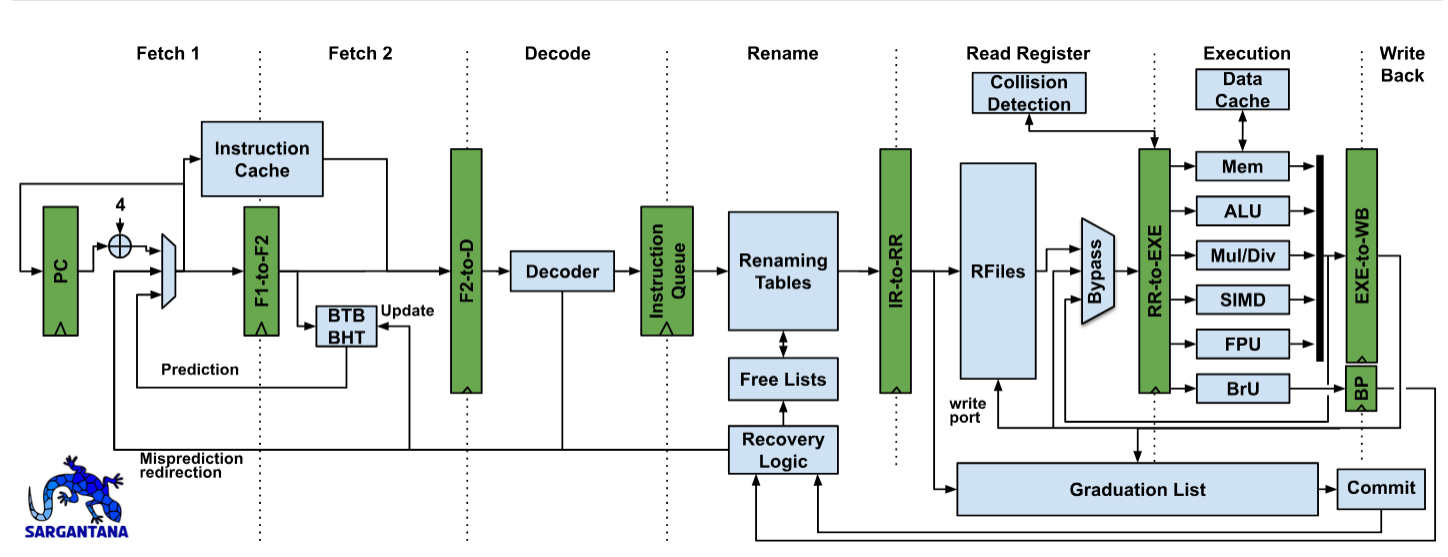
\includegraphics[width=\textwidth]{ch02_pipeline_overview.png}
  \caption{Sargantana complete processor pipeline}
  \label{fig:pipeline-overview}
\end{figure}

The major stages of the pipeline are:

\begin{itemize}
  \item Fetch 1
  \item Fetch 2
  \item Decode
  \item Rename
  \item Register Read
  \item Execution
  \item Write Back
  \item Commit
\end{itemize}

Each stage performs a specific task and communicates with adjacent stages through dedicated
pipeline registers.

\section{Pipeline Stages}

The Sargantana pipeline consists of eight primary stages, each responsible for a particular
phase of instruction execution.

\subsection*{Fetch 1}
The Fetch 1 stage maintains the Program Counter (PC) and communicates with the instruction
cache to request instructions. Branch prediction hardware, including the Branch Target Buffer
(BTB) and Branch History Table (BHT), is also consulted to predict future control flow before
branch instructions are resolved.

\subsection*{Fetch 2}
The second fetch stage receives instructions from the instruction cache and forwards them to
the decode stage through the F2-to-D pipeline register. During this stage, prediction information
generated in Fetch 1 accompanies the fetched instructions.

\subsection*{Decode}
The decode stage interprets the binary instruction encoding and determines:
\begin{itemize}
  \item instruction type
  \item source registers
  \item destination register
  \item immediate values
  \item execution unit selection
  \item control signals
\end{itemize}
The decoded instruction is then inserted into the instruction queue for subsequent processing.

\subsection*{Rename}
One of the defining characteristics of Sargantana is its register renaming stage. Architectural
registers are mapped onto physical registers to eliminate false dependencies such as
Write-After-Write (WAW) and Write-After-Read (WAR) hazards.

This stage also interacts with:
\begin{itemize}
  \item Renaming Tables
  \item Free Lists
  \item Recovery Logic
\end{itemize}
to manage physical register allocation and pipeline recovery following branch mispredictions or
exceptions.

\subsection*{Register Read}
After renaming, source operands are read from the physical register file. If the required
operands have recently been produced but not yet written back, bypass logic forwards the
values directly from later pipeline stages to reduce execution latency.

\subsection*{Execution}
Instructions are dispatched to specialized execution units depending on their operation.
These include:
\begin{itemize}
  \item Arithmetic Logic Unit (ALU)
  \item Branch Unit (BrU)
  \item Load/Store Unit (Memory)
  \item Multiply/Divide Unit
  \item Floating Point Unit (FPU)
  \item SIMD Unit
\end{itemize}
Each functional unit operates independently, allowing several instructions to execute
concurrently.

\subsection*{Write Back}
Upon completion of execution, results are written back into the physical register file. These
results become available for dependent instructions through both register reads and forwarding
paths.

\subsection*{Commit}
Although instructions execute out-of-order, they retire strictly in program order. The commit
stage updates the architectural state only after ensuring that all previous instructions have
completed successfully. This guarantees precise exceptions and preserves program
correctness.

\section{Instruction Flow through the Pipeline}

Figure~\ref{fig:pipeline-overview} illustrates how instructions travel through the processor pipeline.

Unlike an in-order processor, instructions may execute as soon as their operands become
available rather than waiting for older instructions to finish execution. However, all instructions
commit in the original program order, ensuring correct architectural behavior.

\chapter{Top-Level Datapath}

\section{Introduction}

The datapath forms the computational backbone of the Sargantana processor. It interconnects
every major pipeline stage, coordinates the movement of instructions and operands, and
interfaces with all execution units. While the control logic determines \textit{what} operation must be
performed, the datapath determines \textit{where} information flows and \textit{how} the processor state is
updated.

At the highest level, the datapath receives instructions from the instruction fetch subsystem,
processes them through decoding, register renaming, operand reading, execution, and finally
commits the architectural state once execution completes successfully.

The complete organization of the datapath is illustrated in Figure~\ref{fig:datapath-overview}.

\begin{figure}[H]
  \centering
  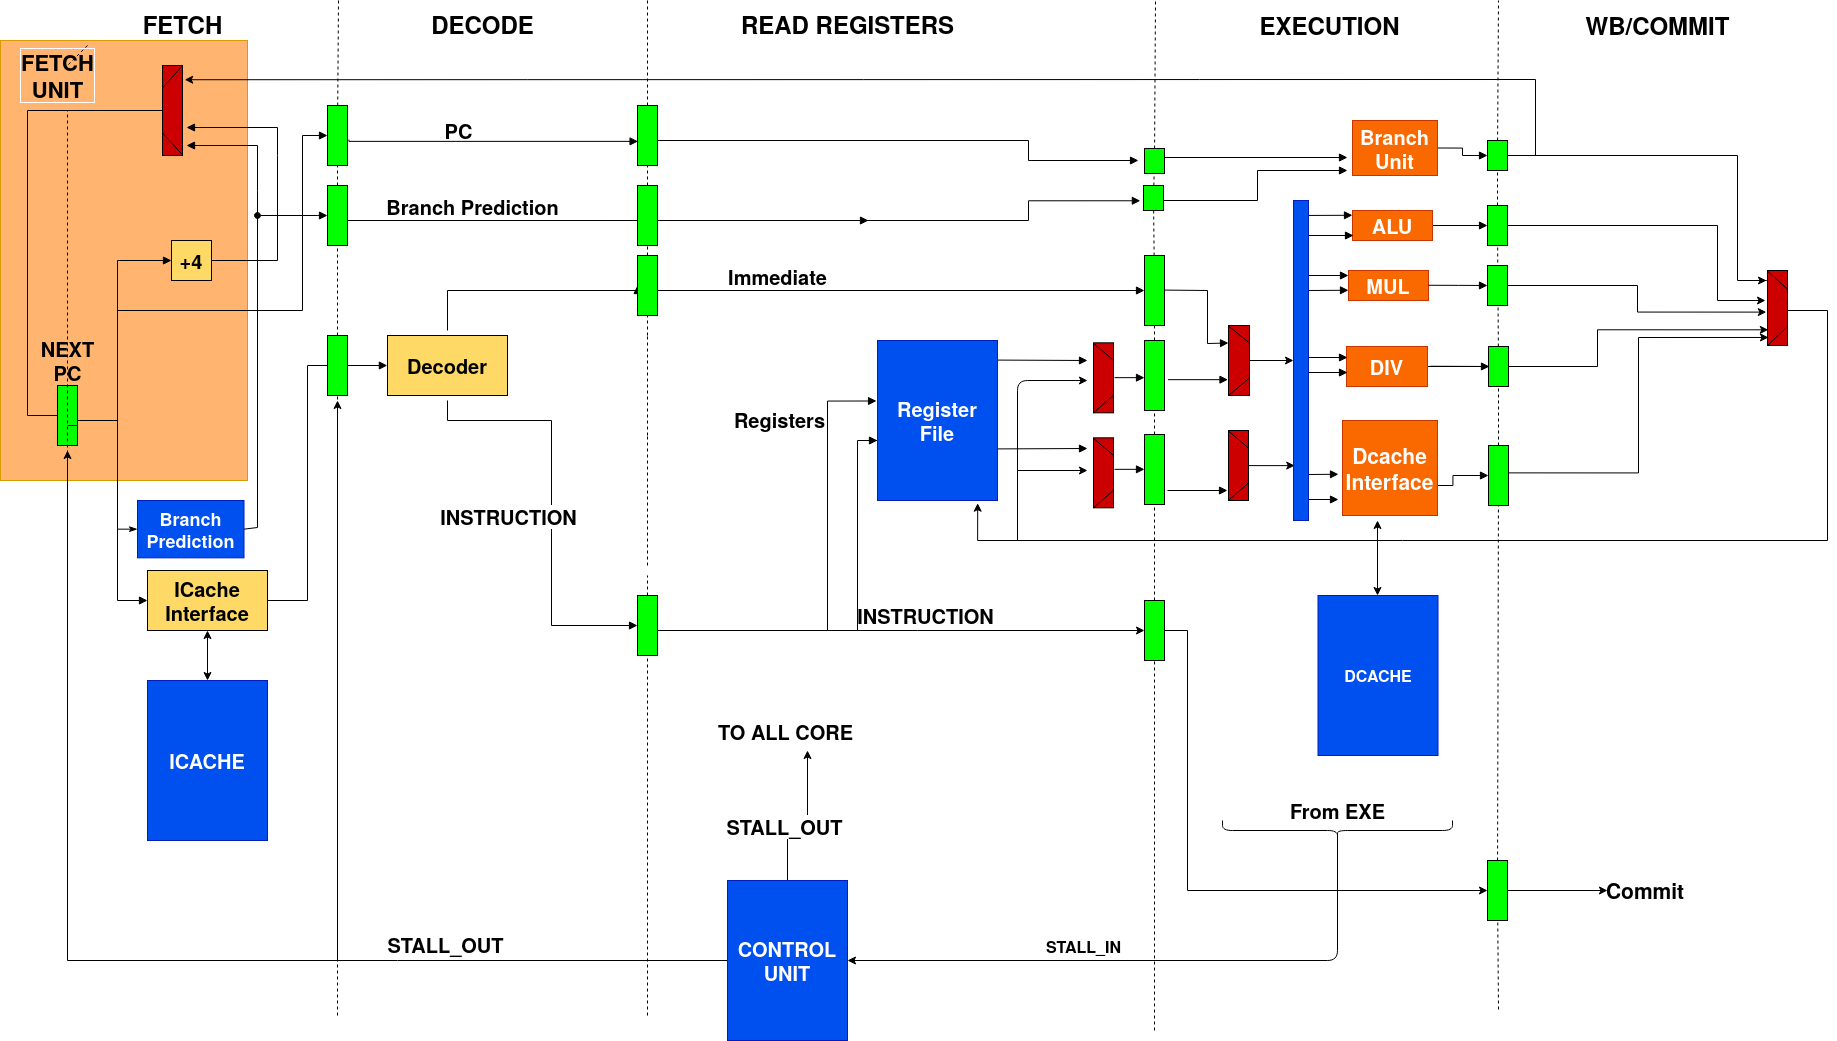
\includegraphics[width=0.85\textwidth]{ch03_datapath_overview.png}
  \caption{Top-level organization of the Sargantana datapath}
  \label{fig:datapath-overview}
\end{figure}

\section{Top-Level Interfaces}

The top-level datapath module serves as the central connection point between the frontend,
backend, execution units, memory subsystem, and commit logic.

Its primary interfaces include:

\subsection*{Instruction Interface}
Receives decoded instructions originating from the frontend pipeline.
Connected modules include:
\begin{itemize}
  \item Decoder
  \item Instruction Queue
\end{itemize}

\subsection*{Register Interface}
Communicates with the physical register file to obtain source operands and write execution
results.
Connected modules include:
\begin{itemize}
  \item Register File
  \item Rename Logic
  \item Bypass Network
\end{itemize}

\subsection*{Execution Interface}
Dispatches instructions to the appropriate execution unit based on the decoded operation.
Supported execution units include:
\begin{itemize}
  \item ALU
  \item Branch Unit
  \item Load/Store Unit
  \item Multiply/Divide Unit
  \item SIMD Unit
  \item Floating Point Unit
\end{itemize}

\subsection*{Commit Interface}
Transfers completed instructions to the Graduation List and Commit stage where architectural
state is updated.

\subsection*{Recovery Interface}
Provides rollback support whenever
\begin{itemize}
  \item branch prediction fails,
  \item exceptions occur,
  \item interrupts arrive.
\end{itemize}
Recovery information is exchanged with the Rename stage and Commit logic to restore a
precise architectural state.

\section{Internal Architecture}

Internally, the datapath acts as the interconnection fabric of the processor.
Instead of implementing computation directly, it instantiates and connects all major pipeline
components.

The internal architecture consists of:
\begin{itemize}
  \item Pipeline Registers
  \item Instruction Queue
  \item Rename Tables
  \item Physical Register File
  \item Bypass Network
  \item Functional Units
  \item Commit Logic
\end{itemize}

\section{Pipeline Registers}

To achieve high throughput, Sargantana separates adjacent pipeline stages using dedicated
pipeline registers.

Important pipeline registers include:
\begin{itemize}
  \item F1-to-F2
  \item F2-to-D
  \item IR-to-RR
  \item RR-to-EXE
  \item EXE-to-WB
\end{itemize}

These registers isolate combinational logic between stages, allowing multiple instructions to
progress simultaneously through different portions of the processor.

\chapter{Instruction Fetch Unit}

\section{Overview}

The Instruction Fetch Unit (IFU) is responsible for supplying a continuous stream of instructions
to the processor pipeline. Its primary responsibilities include maintaining the Program Counter
(PC), accessing the instruction cache, performing branch prediction, and delivering fetched
instructions to the decode stage.

The fetch subsystem is divided into two pipeline stages:
\begin{itemize}
  \item Fetch Stage 1 (F1)
  \item Fetch Stage 2 (F2)
\end{itemize}

This separation enables the processor to overlap instruction fetching with cache access and
branch prediction, thereby improving instruction throughput.

\begin{figure}[h]
  \centering
  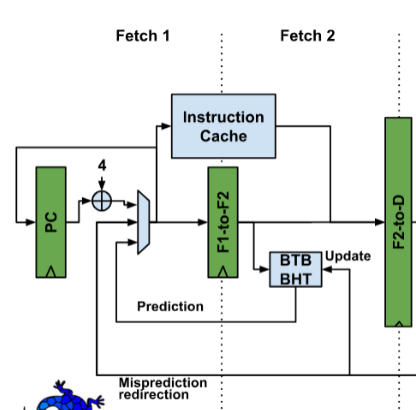
\includegraphics[width=0.75\textwidth]{ch04_fetch_f1_f2.png}
  \caption{Fetch Stage 1 and Fetch Stage 2 organization}
  \label{fig:fetch-f1-f2}
\end{figure}

\section{Program Counter}

The Program Counter (PC) identifies the address of the next instruction to be fetched.
During normal execution, the PC advances sequentially by the instruction width. However, the
fetch stage may also redirect the PC based on:
\begin{itemize}
  \item Branch prediction
  \item Jump instructions
  \item Exceptions
  \item Interrupts
  \item Pipeline recovery after branch misprediction
\end{itemize}

Whenever a branch prediction is later determined to be incorrect, the recovery logic updates the
PC with the correct target address, and instruction fetching resumes from the corrected location.

\section{Fetch Stage 1 (F1)}

Fetch Stage 1 initiates instruction fetching.
Its primary responsibilities include:
\begin{itemize}
  \item Maintaining the Program Counter
  \item Accessing the Branch Target Buffer (BTB)
  \item Reading the Branch History Table (BHT)
  \item Generating prediction information
  \item Sending instruction addresses to the instruction cache
\end{itemize}

This stage attempts to predict future control flow before the instruction has even been decoded,
thereby reducing branch penalties.

\section{Instruction Cache}

The Instruction Cache stores recently accessed instructions to reduce memory access latency.
When Fetch Stage 1 supplies an instruction address, the cache checks whether the
corresponding instruction is already available.

\begin{itemize}
  \item \textbf{Cache Hit:} The instruction is returned immediately.
  \item \textbf{Cache Miss:} The memory hierarchy is accessed to retrieve the required cache line.
\end{itemize}

The instruction cache therefore plays a crucial role in sustaining a high fetch bandwidth and
minimizing pipeline stalls.

\section{Fetch Stage 2 (F2)}

Fetch Stage 2 receives the fetched instruction and associated prediction information from the
instruction cache.

\begin{figure}[h]
  \centering
  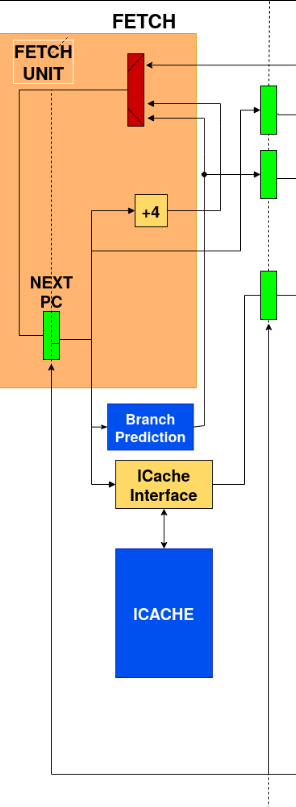
\includegraphics[width=0.45\textwidth]{ch04_fetch_unit_detail.png}
  \caption{Internal detail of the Fetch Unit: PC, +4 adder, ICache interface, and branch prediction}
  \label{fig:fetch-unit-detail}
\end{figure}

Its responsibilities include:
\begin{itemize}
  \item Buffering fetched instructions
  \item Packaging instruction metadata
  \item Forwarding branch prediction information
  \item Passing instructions to the Decode stage via the F2-to-D pipeline register
\end{itemize}

At this point, the instruction has not yet been decoded; it remains in its original binary form.

\chapter{Branch Prediction Subsystem}

\section{Overview}

One of the biggest performance bottlenecks in modern processors is the presence of branch
instructions. Every conditional branch introduces uncertainty because the processor does not
immediately know which instruction should be fetched next. Waiting until the branch is resolved
would stall the pipeline and significantly reduce performance.

To avoid these stalls, Sargantana performs \textbf{speculative execution} by predicting the outcome of
branches before they are executed. If the prediction is correct, instruction execution continues
without interruption. If the prediction is incorrect, speculative instructions are discarded and the
processor restarts from the correct target address.

Unlike a simple five-stage processor, Sargantana performs branch prediction during the
\textbf{Fetch-1 (F1)} stage so that the following stages remain continuously supplied with instructions.

\begin{rtlrefs}
  \rtlitem{rtl/datapath/rtl/if_stage_1/rtl/if_stage_1.sv}
  \rtlitem{rtl/datapath/rtl/if_stage_1/rtl/branch_predictor.sv}
\end{rtlrefs}

\begin{figure}[htbp]
  \centering
  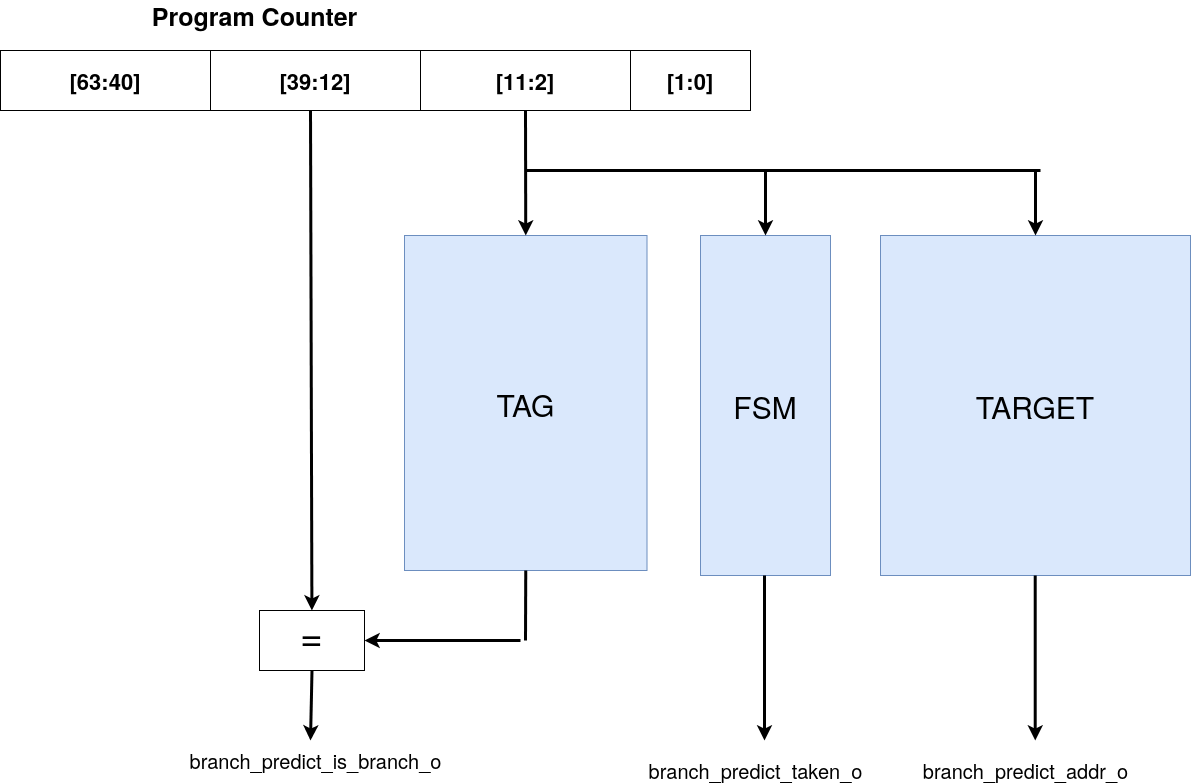
\includegraphics[width=0.68\textwidth]{ch05_btb_bht.png}
  \caption{Program Counter fields feeding the TAG, FSM, and TARGET structures of the branch predictor}
  \label{fig:btb-bht}
\end{figure}

\section{Speculative Execution}

Speculative execution allows instructions located after a predicted branch to begin moving
through the pipeline before the branch outcome is known.

The branch predictor selects one of two possible next PCs:
\begin{itemize}
  \item Sequential PC (PC + 4)
  \item Predicted branch target
\end{itemize}

The Fetch stage immediately begins fetching instructions from the selected address.
If the prediction later proves correct, execution continues normally.
If incorrect, the processor:
\begin{itemize}
  \item flushes incorrect pipeline entries,
  \item restores architectural state,
  \item redirects the PC to the correct target.
\end{itemize}

This recovery mechanism minimizes branch penalties while maintaining correctness.

\begin{rtlrefs}
  \rtlitem{rtl/datapath/rtl/if_stage_1/rtl/if_stage_1.sv}
  \rtlitem{rtl/control_unit/rtl/control_unit.sv}
\end{rtlrefs}

\section{Branch Target Buffer (BTB)}

The Branch Target Buffer stores previously encountered branch instructions together with their
destination addresses.

Whenever a new PC enters Fetch-1, the BTB is searched.
If a matching entry exists, the BTB immediately supplies the predicted destination address
instead of waiting for the branch instruction to execute.

Therefore, BTB answers the question:

\begin{quote}
\textit{``Where should execution go?''}
\end{quote}

Its primary purpose is reducing control hazards caused by indirect and conditional branches.
Within Sargantana, BTB functionality is managed by the branch prediction subsystem inside the
Fetch-1 stage.

\begin{rtlrefs}
  \rtlitem{rtl/datapath/rtl/if_stage_1/rtl/branch_predictor.sv}
\end{rtlrefs}

\section{Branch History Table (BHT)}

Predicting only the target address is insufficient because the processor must also determine
whether the branch will actually be taken.

The Branch History Table records the recent behavior of each branch instruction.
Instead of storing target addresses, it stores prediction information indicating whether the
branch is likely to be:
\begin{itemize}
  \item Taken
  \item Not Taken
\end{itemize}

Sargantana implements this functionality through the Bimodal Predictor, which uses saturating
prediction counters that are continuously updated using previous execution history.

The BHT therefore answers:

\begin{quote}
\textit{``Will this branch be taken?''}
\end{quote}

Together, the BTB and BHT determine both the destination and the likelihood of branching.

\begin{rtlrefs}
  \rtlitem{rtl/datapath/rtl/if_stage_1/rtl/bimodal_predictor.sv}
  \rtlitem{rtl/datapath/rtl/if_stage_1/rtl/branch_predictor.sv}
\end{rtlrefs}

\section{Return Address Stack (RAS)}

Function calls and returns occur very frequently in software.
Predicting return instructions using only the BTB is often inaccurate because a single function
may be called from many different locations.

To improve prediction accuracy, Sargantana implements a Return Address Stack (RAS).

Operation:
\begin{itemize}
  \item CALL instruction $\rightarrow$ push return address.
  \item RETURN instruction $\rightarrow$ pop return address.
  \item popped address becomes predicted next PC.
\end{itemize}

This significantly improves prediction accuracy for nested function calls.

The Return Address Stack is implemented as an independent hardware structure inside the
Fetch stage.

\begin{rtlrefs}
  \rtlitem{rtl/datapath/rtl/if_stage_1/rtl/return_address_stack.sv}
\end{rtlrefs}

\section{Prediction Flow}

The overall prediction process performed during instruction fetch is summarized below.

\begin{enumerate}
  \item Current Program Counter enters Fetch-1.
  \item Branch Predictor receives the PC.
  \item BTB checks whether the PC corresponds to a known branch.
  \item BHT predicts whether the branch will be taken.
  \item RAS provides return addresses for function returns when required.
  \item Predictor selects the next PC.
  \item Fetch-2 retrieves instructions from the predicted address.
  \item Later execution stages verify the correctness of the prediction.
  \item If incorrect, Recovery Logic flushes the pipeline and redirects execution.
\end{enumerate}

This mechanism allows Sargantana to maintain a high instruction throughput while minimizing
branch penalties.

\begin{rtlrefs}
  \rtlitem{rtl/datapath/rtl/if_stage_1/rtl/if_stage_1.sv}
  \rtlitem{rtl/datapath/rtl/if_stage_1/rtl/branch_predictor.sv}
  \rtlitem{rtl/control_unit/rtl/control_unit.sv}
\end{rtlrefs}

\section{Recovery from Mispredictions}

A branch prediction is considered complete only after the branch instruction executes.
If the prediction matches the actual result, execution proceeds normally.
Otherwise, the processor performs a recovery sequence:

\begin{itemize}
  \item Flush speculative instructions.
  \item Restore the correct architectural state.
  \item Update predictor history.
  \item Redirect the Program Counter.
  \item Resume instruction fetch.
\end{itemize}

The recovery logic works together with:
\begin{itemize}
  \item Instruction Queue
  \item Rename Tables
  \item Free Lists
  \item Graduation List
  \item Control Unit
\end{itemize}

to ensure that incorrectly executed speculative instructions never modify the committed
architectural state.

\begin{rtlrefs}
  \rtlitem{rtl/control_unit/rtl/control_unit.sv}
  \rtlitem{rtl/datapath/rtl/ir_stage/rtl/instruction_queue.sv}
  \rtlitem{rtl/datapath/rtl/ir_stage/rtl/rename_table.sv}
  \rtlitem{rtl/datapath/rtl/ir_stage/rtl/free_list.sv}
  \rtlitem{rtl/datapath/rtl/wb_stage/rtl/graduation_list.sv}
\end{rtlrefs}

\chapter{Decode Stage}

\section{Overview}

The Decode stage receives fetched instructions from Fetch-2 and converts them into an internal
representation suitable for later pipeline stages.

Its responsibilities include:
\begin{itemize}
  \item decoding the instruction opcode,
  \item extracting source and destination registers,
  \item generating immediate values,
  \item identifying instruction formats,
  \item producing control information,
  \item forwarding decoded instructions to the Rename stage.
\end{itemize}

This stage forms the interface between instruction fetch and out-of-order execution.

\begin{rtlrefs}
  \rtlitem{rtl/datapath/rtl/id_stage/rtl/decoder.sv}
  \rtlitem{rtl/datapath/rtl/id_stage/rtl/immediate.sv}
\end{rtlrefs}

\begin{figure}[htbp]
  \centering
  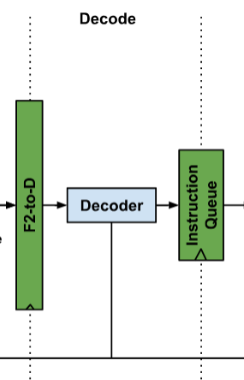
\includegraphics[width=0.28\textwidth]{ch06_decode_overview.png}
  \caption{Decode stage: F2-to-D $\rightarrow$ Decoder $\rightarrow$ Instruction Queue}
  \label{fig:decode-overview}
\end{figure}

\begin{figure}[htbp]
  \centering
  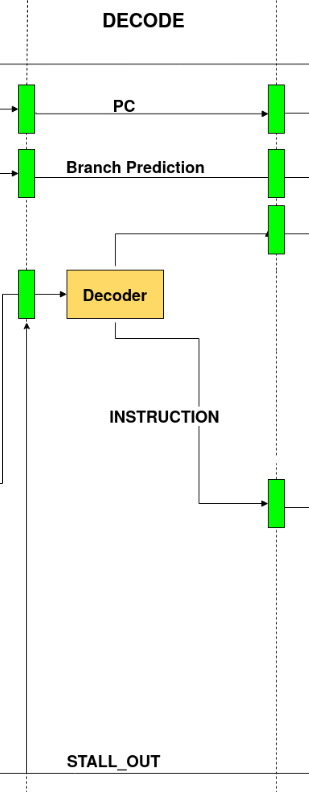
\includegraphics[width=0.26\textwidth]{ch06_decode_detail.png}
  \caption{Detailed signal view of the Decode stage}
  \label{fig:decode-detail}
\end{figure}

\section{Instruction Decode}

The Decoder interprets the binary instruction according to the RISC-V ISA.
It identifies:
\begin{itemize}
  \item instruction format,
  \item functional unit,
  \item register operands,
  \item immediate usage,
  \item memory operations,
  \item branch instructions,
  \item CSR accesses,
  \item floating-point instructions,
  \item vector instructions.
\end{itemize}

The decoded information is forwarded toward Rename.

\begin{rtlrefs}
  \rtlitem{rtl/datapath/rtl/id_stage/rtl/decoder.sv}
\end{rtlrefs}

\section{Immediate Generation}

Many RISC-V instructions contain embedded immediate fields.
The Immediate Generator extracts these fields and reconstructs complete signed values
according to the instruction format.

Supported formats include:
\begin{itemize}
  \item I-type
  \item S-type
  \item B-type
  \item U-type
  \item J-type
\end{itemize}

These immediates are later consumed by the ALU, Branch Unit, and Address Generation Unit.

\begin{rtlrefs}
  \rtlitem{rtl/datapath/rtl/id_stage/rtl/immediate.sv}
\end{rtlrefs}

\section{Opcode Decoding}

Opcode decoding determines the exact class of instruction.
Examples include:
\begin{itemize}
  \item Arithmetic
  \item Logical
  \item Branch
  \item Jump
  \item Load
  \item Store
  \item Floating Point
  \item SIMD
  \item CSR
  \item System
\end{itemize}

The Decoder produces internal control signals used by downstream stages to select the
appropriate execution unit.

\begin{rtlrefs}
  \rtlitem{rtl/datapath/rtl/id_stage/rtl/decoder.sv}
\end{rtlrefs}

\section{Control Signal Generation}

Based on the decoded instruction, the Decode stage generates the control information required
throughout the remainder of the pipeline.

These signals specify:
\begin{itemize}
  \item destination register validity,
  \item operand selection,
  \item ALU operation,
  \item branch type,
  \item memory access type,
  \item CSR operation,
  \item vector operation,
  \item floating-point operation.
\end{itemize}

These control signals accompany the instruction into the Rename stage.

\begin{rtlrefs}
  \rtlitem{rtl/datapath/rtl/id_stage/rtl/decoder.sv}
  \rtlitem{rtl/control_unit/rtl/control_unit.sv}
\end{rtlrefs}

\section{Output to Rename Stage}

After decoding completes, the instruction is forwarded to the Rename stage.

At this point the instruction has:
\begin{itemize}
  \item decoded opcode,
  \item source registers,
  \item destination register,
  \item immediate value,
  \item generated control signals.
\end{itemize}

The Rename stage will subsequently eliminate false register dependencies using register
renaming before dispatching instructions toward execution.

\begin{rtlrefs}
  \rtlitem{rtl/datapath/rtl/id_stage/rtl/decoder.sv}
  \rtlitem{rtl/datapath/rtl/ir_stage/rtl/rename_table.sv}
  \rtlitem{rtl/datapath/rtl/ir_stage/rtl/instruction_queue.sv}
\end{rtlrefs}

\begin{figure}[htbp]
  \centering
  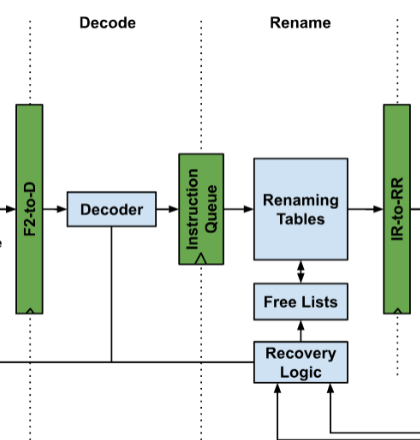
\includegraphics[width=0.55\textwidth]{ch06_decode_to_rename.png}
  \caption{Decoded instructions flowing from the Decode stage into the Rename stage}
  \label{fig:decode-to-rename}
\end{figure}

\subsection*{Example (adapted from \texttt{doc/specification/decoder\_specification})}

The cases are:

\begin{itemize}
  \item Cycle 1: Invalid input $\rightarrow$ invalid output.
  \item Cycle 2: Exception input $\rightarrow$ exception output and not decoded.
  \item Cycle 3: Regular case, valid input, not illegal instruction, and signed operation.
  \item Cycle 4: Regular case again, but it has the power to change the PC.
  \item Cycle 5: Case with illegal instruction, hence exception valid to 1.
  \item Cycle 6: Case of the fence with the special signal to 1.
\end{itemize}

In the following figure we can see all the cases mentioned above.

\begin{figure}[htbp]
  \centering
  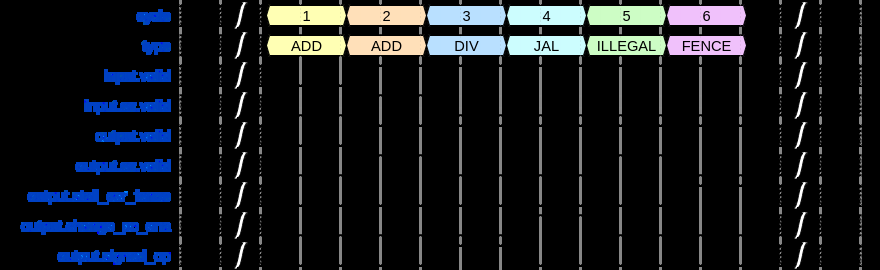
\includegraphics[width=\textwidth]{ch06_decoder_waveform.png}
  \caption{Decoder timing waveform illustrating the six example cases}
  \label{fig:decoder-waveform}
\end{figure}

\chapter{Register Rename Stage}

\section{Overview}

After an instruction has been decoded, it enters the Register Rename (IR) stage. The primary
objective of this stage is to eliminate false dependencies caused by reuse of architectural
register names.

In the Sargantana processor, the rename stage consists of three major components:
\begin{itemize}
  \item Register Alias Table (Rename Table)
  \item Free List
  \item Instruction Queue
\end{itemize}

These modules are implemented in:

\begin{center}
\rtl{rtl/datapath/rtl/ir\_stage/}
\end{center}

Important RTL files include:

\begin{rtlrefs}
  \rtlitem{rtl/datapath/rtl/ir_stage/rtl/rename_table.sv}
  \rtlitem{rtl/datapath/rtl/ir_stage/rtl/free_list.sv}
  \rtlitem{rtl/datapath/rtl/ir_stage/rtl/instruction_queue.sv}
\end{rtlrefs}

\begin{figure}[H]
  \centering
  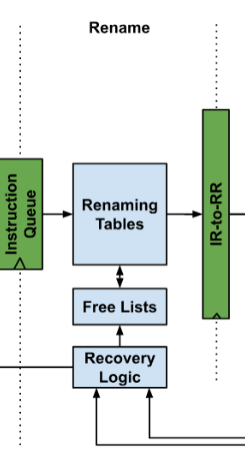
\includegraphics[width=0.33\textwidth]{ch07_rename_overview.png}
  \caption{Rename stage: Instruction Queue, Renaming Tables, Free Lists, and Recovery Logic}
  \label{fig:rename-overview}
\end{figure}

\section{Register Renaming}

Modern superscalar processors allow multiple instructions to execute simultaneously. If two
instructions write to the same architectural register, false dependencies arise even when the
instructions are logically independent.

Register renaming solves this problem by mapping architectural registers onto a much larger
pool of physical registers.

For example:
\begin{verbatim}
ADD x5, x1, x2
SUB x5, x3, x4
\end{verbatim}

Architecturally, both instructions write to \texttt{x5}.

\textbf{Without renaming:}
\begin{verbatim}
ADD -----> x5
SUB -----> x5
\end{verbatim}
The second instruction must wait.

\textbf{With renaming:}
\begin{verbatim}
ADD -----> P17
SUB -----> P22
\end{verbatim}
Both instructions can execute independently.

This mapping is maintained inside:

\begin{center}
\rtl{rtl/datapath/rtl/ir\_stage/rtl/rename\_table.sv}
\end{center}

\section{Register Alias Table (RAT)}

The Register Alias Table (RAT), implemented as the Rename Table, stores the current mapping
between architectural registers and physical registers.

Rather than reading an architectural register directly, later stages first consult the Rename Table
to determine which physical register currently holds the latest value.

Whenever a new destination register is renamed, the table updates its mapping.

The implementation resides in:

\begin{center}
\rtl{rtl/datapath/rtl/ir\_stage/rtl/rename\_table.sv}
\end{center}

The Rename Table therefore becomes the central structure responsible for maintaining correct
register mappings throughout speculative execution.

\section{Physical Register Allocation}

Each new destination register requires a free physical register.

Instead of searching all registers every cycle, Sargantana maintains a dedicated Free List.

The Free List keeps track of unused physical registers.

Whenever an instruction requires a destination register, the allocation proceeds as shown below.

\begin{figure}[H]
  \centering
  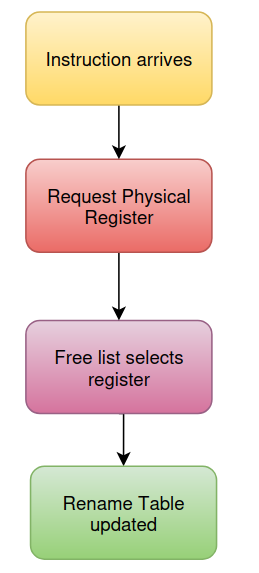
\includegraphics[width=0.3\textwidth]{ch07_physical_register_allocation.png}
  \caption{Physical register allocation flow: Instruction arrives $\rightarrow$ Request Physical Register $\rightarrow$ Free List selects register $\rightarrow$ Rename Table updated}
  \label{fig:phys-reg-alloc}
\end{figure}

When an instruction finally commits, its old physical register is returned to the Free List for
reuse.

This functionality is implemented in:

\begin{center}
\rtl{rtl/datapath/rtl/ir\_stage/rtl/free\_list.sv}
\end{center}

Together, the Free List and Rename Table enable efficient dynamic register allocation.

\section{Hazard Elimination}

The rename stage primarily eliminates false dependencies:
\begin{itemize}
  \item Write After Write (WAW)
  \item Write After Read (WAR)
\end{itemize}

Because each destination register receives a unique physical register, later instructions no
longer overwrite the results of earlier instructions.

Only true data dependencies (RAW) remain.

The renamed instructions are temporarily stored inside the Instruction Queue before being
issued to the Register Read stage.

Instruction Queue implementation:

\begin{center}
\rtl{rtl/datapath/rtl/ir\_stage/rtl/instruction\_queue.sv}
\end{center}

The rename stage therefore prepares instructions for high-performance out-of-order execution
while maintaining correct architectural state.

\chapter{Register Read Stage}

\section{Overview}

Following register renaming, instructions enter the Register Read (RR) stage. At this point, all
architectural register references have already been converted into physical register identifiers.

The purpose of this stage is to obtain the actual operand values required for execution.

In Sargantana, the Register Read stage is centered around the physical register file.

RTL location:

\begin{center}
\rtl{rtl/datapath/rtl/rr\_stage/}
\end{center}

Primary implementation:

\begin{center}
\rtl{rtl/datapath/rtl/rr\_stage/rtl/regfile.sv}
\end{center}

This stage receives renamed instructions from the Rename stage and forwards operand values
toward the Execution stage.

\begin{figure}[h]
  \centering
  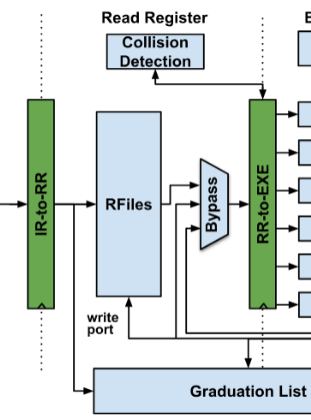
\includegraphics[width=0.5\textwidth]{ch08_register_read_overview.png}
  \caption{Register Read stage: RFiles, Bypass, and Collision Detection}
  \label{fig:register-read-overview}
\end{figure}

\section{Register File}

The register file stores all physical register values currently available inside the processor.
Unlike a simple in-order processor, the register file is accessed using physical register numbers
generated during register renaming.

The module is implemented in:

\begin{center}
\rtl{rtl/datapath/rtl/rr\_stage/rtl/regfile.sv}
\end{center}

The register file supports:
\begin{itemize}
  \item Reading source operands
  \item Writing completed results back into physical registers
  \item Supplying operands to multiple execution units
\end{itemize}

This module serves as the central storage element for operand values.

\section{Operand Read}

Once physical register identifiers are available, the register file reads the corresponding operand
values.

For an instruction:
\begin{verbatim}
ADD P17, P4, P8
\end{verbatim}

the Register Read stage performs:
\begin{verbatim}
Read P4
Read P8
  |
Operand A
Operand B
  |
Execution Stage
\end{verbatim}

This process occurs every cycle for all issued instructions.

The implementation is handled by:

\begin{center}
\rtl{rtl/datapath/rtl/rr\_stage/rtl/regfile.sv}
\end{center}

\section{Operand Forwarding}

Waiting for every instruction to write back before reading operands would significantly reduce
performance. To minimize stalls, recently computed values may be forwarded directly from
execution units.

\begin{figure}[h]
  \centering
  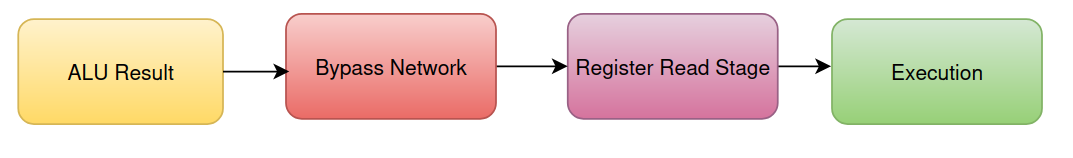
\includegraphics[width=\textwidth]{ch08_bypass_network.png}
  \caption{Conceptual bypass path: ALU Result $\rightarrow$ Bypass Network $\rightarrow$ Register Read Stage $\rightarrow$ Execution}
  \label{fig:bypass-network}
\end{figure}

The pipeline overview shows this Bypass path between the Register Read and Execution
stages.

Although the forwarding logic spans multiple execution modules, the Register Read stage is
designed to receive these forwarded values whenever available.

\section{Dependency Resolution}

Even after register renaming, true data dependencies (Read After Write) must still be respected.

The Register Read stage ensures that:
\begin{itemize}
  \item Ready operands are immediately read from the register file.
  \item Forwarded operands are used whenever newer values exist.
  \item Instructions with unresolved dependencies wait until their operands become available.
\end{itemize}

Once all operands are available, the instruction advances to the Execution stage, where
arithmetic, logical, memory, floating-point, SIMD, or branch operations are performed.

The interaction between Register Read and Execution is coordinated through:

\begin{center}
\rtl{rtl/datapath/rtl/datapath.sv}
\end{center}

and the execution subsystem rooted at:

\begin{center}
\rtl{rtl/datapath/rtl/exe\_stage/rtl/exe\_stage.sv}
\end{center}

This completes the front-end portion of the Sargantana datapath before execution begins.

\chapter{Execution Stage}

\section{Overview}

The Execution (EXE) stage is responsible for performing the actual computation requested by
each instruction. After operands have been read from the physical register file, instructions are
dispatched to the appropriate execution unit based on their operation type.

Unlike a simple in-order processor that contains a single ALU, Sargantana contains multiple
specialized execution units capable of executing integer, branch, multiplication, division,
floating-point, SIMD and memory operations simultaneously.

The entire execution subsystem is implemented under:

\begin{center}
\rtldir{rtl/datapath/rtl/exe\_stage/}
\end{center}

The top-level execution module is:

\begin{center}
\rtl{rtl/datapath/rtl/exe\_stage/rtl/exe\_stage.sv}
\end{center}

This module acts as the dispatcher for all execution units and interfaces with the Load/Store
subsystem, scoreboards, writeback logic and pipeline control.

\begin{figure}[htbp]
  \centering
  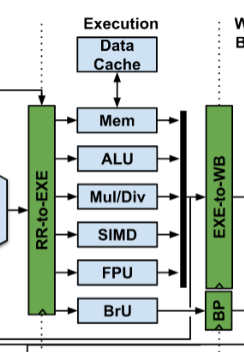
\includegraphics[width=0.43\textwidth]{ch09_execution_overview.png}
  \caption{Execution stage overview: RR-to-EXE dispatch to Mem, ALU, Mul/Div, SIMD, FPU, and BrU}
  \label{fig:execution-overview}
\end{figure}

\section{Arithmetic Logic Unit (ALU)}

The Arithmetic Logic Unit performs all integer arithmetic and logical operations. Instead of
implementing every operation inside one large module, Sargantana divides the ALU into several
dedicated functional blocks.

The top-level ALU is implemented in:

\begin{center}
\rtl{rtl/datapath/rtl/exe\_stage/rtl/alu/alu.sv}
\end{center}

Internally, the ALU is divided into the following modules:

\begin{longtable}{@{}p{0.45\textwidth}p{0.5\textwidth}@{}}
\toprule
\textbf{RTL File} & \textbf{Function} \\
\midrule
\endhead
\rtlx{alu\_add.sv}{rtl/datapath/rtl/exe_stage/rtl/alu/alu_add.sv} & Addition and subtraction \\
\rtlx{alu\_logic.sv}{rtl/datapath/rtl/exe_stage/rtl/alu/alu_logic.sv} & AND, OR, XOR operations \\
\rtlx{alu\_shift.sv}{rtl/datapath/rtl/exe_stage/rtl/alu/alu_shift.sv} & Logical and arithmetic shifts \\
\rtlx{alu\_cmp.sv}{rtl/datapath/rtl/exe_stage/rtl/alu/alu_cmp.sv} & Comparison instructions (SLT, SLTU, etc.) \\
\rtlx{alu\_count\_pop.sv}{rtl/datapath/rtl/exe_stage/rtl/alu/alu_count_pop.sv} & Population count instructions \\
\rtlx{zero\_counter/alu\_count\_zeros.sv}{rtl/datapath/rtl/exe_stage/rtl/alu/zero_counter/alu_count_zeros.sv} & Leading/trailing zero count operations \\
\bottomrule
\end{longtable}

This modular implementation simplifies verification while allowing new ALU extensions to be
integrated independently.

\section{Branch Unit}

Branch instructions require a different execution path than arithmetic instructions because they
determine the next program counter value.

The Branch Unit performs:
\begin{itemize}
  \item Conditional branch evaluation
  \item Branch target calculation
  \item Branch taken/not-taken decision
  \item Branch misprediction recovery support
\end{itemize}

RTL implementation:

\begin{center}
\rtl{rtl/datapath/rtl/exe\_stage/rtl/branch\_unit.sv}
\end{center}

Although branch prediction occurs during the fetch stage, the Branch Unit provides the final
verification of branch outcomes during execution. Any prediction mismatch is reported back to
the pipeline so that incorrect speculative instructions can be flushed.

\section{Multiplier Unit}

Integer multiplication operations are handled by a dedicated multiplier unit.

RTL implementation:

\begin{center}
\rtl{rtl/datapath/rtl/exe\_stage/rtl/mul\_unit.sv}
\end{center}

Separating multiplication from the ALU allows multiplication instructions to execute
independently without increasing the critical path of simple arithmetic operations.

The multiplier supports RISC-V integer multiplication instructions while integrating with the
pipeline's scoreboard and scheduling logic.

\section{Divider Unit}

Division operations typically require multiple clock cycles and therefore utilize a dedicated
hardware divider.

The Divider subsystem consists of:

\begin{rtlrefs}
  \rtlitem{rtl/datapath/rtl/exe_stage/rtl/div_unit.sv}
  \rtlitem{rtl/datapath/rtl/exe_stage/rtl/div_4bits.sv}
\end{rtlrefs}

The divider performs integer division and remainder calculations while allowing the processor to
continue issuing independent instructions. The scoreboard tracks outstanding division
operations until completion.

\section{Memory Unit}

Load and store instructions are processed by the Memory Unit, which interfaces directly with the
Load/Store Queue and the cache subsystem.

Primary RTL modules include:

\begin{rtlrefs}
  \rtlitem{rtl/datapath/rtl/exe_stage/rtl/mem_unit.sv}
  \rtlitem{rtl/datapath/rtl/exe_stage/rtl/load_store_queue.sv}
  \rtlitem{rtl/datapath/rtl/exe_stage/rtl/store_buffer.sv}
  \rtlitem{rtl/datapath/rtl/exe_stage/rtl/vagu.sv}
\end{rtlrefs}

The responsibilities of these modules include:
\begin{itemize}
  \item Effective address calculation
  \item Load request generation
  \item Store buffering
  \item Memory dependency handling
  \item Interface with the memory hierarchy
\end{itemize}

The dedicated Address Generation Unit (\rtlx{vagu.sv}{rtl/datapath/rtl/exe_stage/rtl/vagu.sv}) computes effective memory addresses
before memory accesses are issued.

\section{Execution Pipeline Flow}

Once an instruction reaches the Execution stage, it is dispatched to the appropriate functional
unit according to its opcode.

The execution flow can be summarized as shown in Figure~\ref{fig:execution-flow}.

\begin{figure}[htbp]
  \centering
  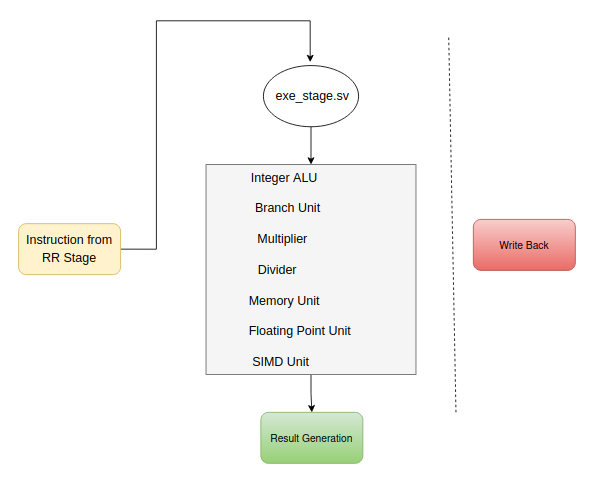
\includegraphics[width=0.6\textwidth]{ch09_execution_pipeline_flow.png}
  \caption{Execution pipeline flow: dispatch through \texttt{exe\_stage.sv} to the functional units and result generation}
  \label{fig:execution-flow}
\end{figure}

The execution stage also integrates several auxiliary modules that coordinate long-latency
operations:

\begin{rtlrefs}
  \rtlitemx{pending_mem_req_queue.sv}{rtl/datapath/rtl/exe_stage/rtl/pending_mem_req_queue.sv}
  \rtlitemx{pending_fp_ops_queue.sv}{rtl/datapath/rtl/exe_stage/rtl/pending_fp_ops_queue.sv}
  \rtlitemx{score_board_scalar.sv}{rtl/datapath/rtl/exe_stage/rtl/score_board_scalar.sv}
  \rtlitemx{score_board_simd.sv}{rtl/datapath/rtl/exe_stage/rtl/score_board_simd.sv}
\end{rtlrefs}

These modules allow Sargantana to support out-of-order execution while maintaining correct
instruction dependencies.

\begin{figure}[htbp]
  \centering
  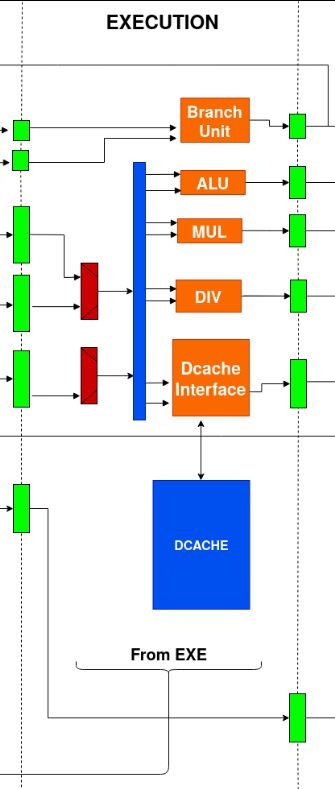
\includegraphics[width=0.28\textwidth]{ch09_execution_detail.png}
  \caption{Detailed execution-stage datapath, including the D-cache interface and auxiliary queues}
  \label{fig:execution-detail}
\end{figure}

\begin{quote}
\textit{Note: it was refined later on, I guess, because the current pipeline is a bit more advanced!}
\end{quote}

\chapter{Memory Subsystem}

\section{Overview}

The Memory Subsystem manages all load and store operations generated by the processor.
Rather than accessing memory directly from the execution stage, Sargantana uses dedicated
hardware structures to support efficient memory scheduling, dependency tracking and store
buffering.

The primary RTL modules involved in memory operations are:

\begin{rtlrefs}
  \rtlitem{rtl/datapath/rtl/exe_stage/rtl/mem_unit.sv}
  \rtlitem{rtl/datapath/rtl/exe_stage/rtl/load_store_queue.sv}
  \rtlitem{rtl/datapath/rtl/exe_stage/rtl/store_buffer.sv}
  \rtlitem{rtl/datapath/rtl/exe_stage/rtl/vagu.sv}
  \rtlitem{rtl/datapath/rtl/interface_csr/rtl/csr_interface.sv}
\end{rtlrefs}

These modules collectively implement the processor's memory execution pipeline.

\section{Load Operations}

When a load instruction reaches the Execution stage, the effective address is first computed by
the Address Generation Unit (\rtl{vagu.sv}). The request is then inserted into the Load/Store
Queue, which manages pending memory operations.

The Memory Unit (\rtl{mem\_unit.sv}) communicates with the cache hierarchy and retrieves the
requested data. Once the data becomes available, it is forwarded toward the Writeback stage,
where it updates the corresponding physical register.

This separation allows multiple outstanding memory requests to be tracked without stalling the
entire pipeline.

\section{Store Operations}

Store instructions follow a similar flow but differ in that they write data to memory rather than
returning a result to the register file.

Before a store is committed to memory, it is temporarily held in the Store Buffer:

\begin{center}
\rtl{rtl/datapath/rtl/exe\_stage/rtl/store\_buffer.sv}
\end{center}

The Store Buffer allows execution to continue while pending store operations are safely queued.
Once it is safe to update memory, buffered store entries are committed in program order.

\section{Address Generation}

Effective memory addresses are generated by the dedicated Address Generation Unit.

RTL implementation:

\begin{center}
\rtl{rtl/datapath/rtl/exe\_stage/rtl/vagu.sv}
\end{center}

The Address Generation Unit combines the base register value with the instruction offset to
compute the final virtual address used by both load and store operations.

Separating address generation into its own module improves modularity and enables future
support for more advanced addressing modes.

\section{Cache Interface}

The Memory Unit serves as the interface between the execution pipeline and the processor's
cache hierarchy. It issues memory requests generated by the Load/Store Queue and receives
the corresponding responses.

The cache interface logic is primarily coordinated by:

\begin{center}
\rtl{rtl/datapath/rtl/exe\_stage/rtl/mem\_unit.sv}
\end{center}

and integrated into the top-level datapath through:

\begin{center}
\rtl{rtl/datapath/rtl/datapath.sv}
\end{center}

This organization isolates cache communication from the rest of the execution logic while
allowing memory latency to be managed independently.

\section{Memory Ordering}

Correct program execution requires that memory operations observe architectural ordering
rules. Sargantana enforces this through the interaction of the Load/Store Queue, Store Buffer
and scoreboard structures.

The relevant RTL modules include:

\begin{rtlrefs}
  \rtlitem{load_store_queue.sv}
  \rtlitem{store_buffer.sv}
  \rtlitem{pending_mem_req_queue.sv}
  \rtlitem{score_board_scalar.sv}
\end{rtlrefs}

Together, these modules track outstanding memory requests, preserve dependencies between
loads and stores, and ensure that memory operations are completed in a correct and consistent
order before instructions are retired.

\chapter{Writeback Stage}

\section{Overview}

The Writeback (WB) stage is responsible for collecting the completed results produced by the
execution units and making them available for architectural retirement. Unlike an in-order
processor where results are written directly into the register file, Sargantana employs an
out-of-order backend. Consequently, completed execution results are first gathered and
associated with their corresponding physical registers before the instruction becomes eligible for
retirement.

The writeback stage therefore acts as the interface between execution and commit. It receives
completion notifications from multiple functional units such as the ALU, multiplier, divider,
floating-point unit, SIMD unit, and memory subsystem. Once a result is available, the stage
updates the internal completion status so that dependent instructions may proceed and the
commit stage can eventually retire the instruction.

Unlike the execution stage, the writeback logic mainly manages completed instruction
information rather than performing arithmetic computations.

\begin{rtlrefs}
  \rtlitem{rtl/datapath/rtl/wb_stage/rtl/graduation_list.sv}
  \rtlitem{rtl/datapath/rtl/datapath.sv}
\end{rtlrefs}

\begin{figure}[H]
  \centering
  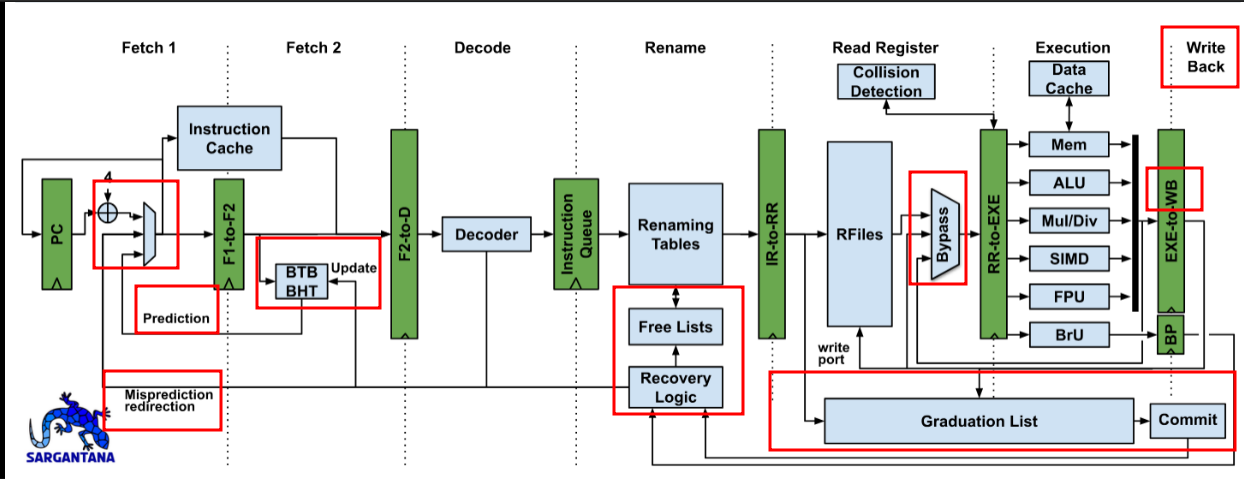
\includegraphics[width=\textwidth]{ch11_writeback_overview.png}
  \caption{Writeback stage in context: results flow from the execution units into the Graduation List and Commit}
  \label{fig:writeback-overview}
\end{figure}

\section{Result Collection}

Multiple execution units operate simultaneously and may finish execution at different clock
cycles. The writeback stage therefore collects completed results from all available execution
pipelines.

Typical producers include:
\begin{itemize}
  \item Integer ALU
  \item Branch Unit
  \item Multiplier
  \item Divider
  \item Memory Unit
  \item Floating Point Unit
  \item SIMD Unit
\end{itemize}

\begin{figure}[H]
  \centering
  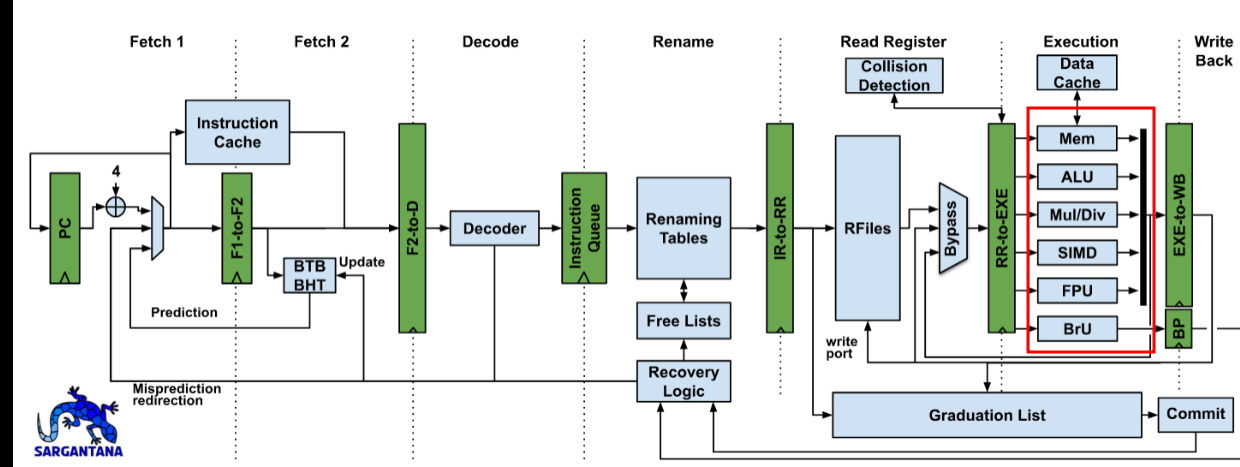
\includegraphics[width=\textwidth]{ch11_result_collection.png}
  \caption{Result collection: completed results from the highlighted execution units feed the writeback stage}
  \label{fig:result-collection}
\end{figure}

Each completed instruction provides:
\begin{itemize}
  \item Destination physical register
  \item Computed result
  \item Completion indication
  \item Exception information (if generated)
\end{itemize}

Rather than immediately committing the instruction, the writeback stage records that the
instruction has completed successfully.

The RTL implements this functionality through the \textbf{Graduation List}, which keeps track of
instructions that have completed execution and are waiting for architectural retirement.

\begin{rtlrefs}
  \rtlitem{rtl/datapath/rtl/wb_stage/rtl/graduation_list.sv}
\end{rtlrefs}

\section{Register Update}

Because Sargantana uses physical register renaming, execution results are written into the
allocated physical register instead of directly updating the architectural register file.

The sequence is:
\begin{enumerate}
  \item Register Rename allocates a physical register.
  \item Execution computes the instruction result.
  \item Writeback stores the value into the physical register.
  \item Commit later updates the architectural mapping.
\end{enumerate}

This separation allows speculative instructions to execute safely without modifying the visible
architectural state.

The Graduation List maintains the completion status for each instruction until the Commit stage
verifies that the instruction can safely retire.

This mechanism supports:
\begin{itemize}
  \item speculative execution
  \item precise exceptions
  \item rollback after branch misprediction
  \item correct in-order retirement
\end{itemize}

\begin{rtlrefs}
  \rtlitem{rtl/datapath/rtl/ir_stage/rtl/rename_table.sv}
  \rtlitem{rtl/datapath/rtl/rr_stage/rtl/regfile.sv}
  \rtlitem{rtl/datapath/rtl/wb_stage/rtl/graduation_list.sv}
\end{rtlrefs}

\section{Exception Information}

Besides carrying execution results, the writeback stage also forwards exception information
generated during execution.

Examples include:
\begin{itemize}
  \item Illegal instruction
  \item Load or Store access fault
  \item Misaligned memory access
  \item Arithmetic exceptions
  \item Floating-point exceptions
\end{itemize}

Instead of immediately servicing an exception, the writeback stage records the exception status
alongside the completed instruction.

The Commit stage later checks whether the faulting instruction is the oldest instruction in the
machine. Only then is the architectural state updated and the exception is delivered,
guaranteeing precise exception handling.

This approach ensures that younger speculative instructions never modify architectural state
before older instructions have safely completed.

\begin{rtlrefs}
  \rtlitem{rtl/datapath/rtl/wb_stage/rtl/graduation_list.sv}
  \rtlitem{rtl/control_unit/rtl/control_unit.sv}
\end{rtlrefs}

\chapter{Commit Stage}

\section{Overview}

The Commit stage is the final stage of the Sargantana pipeline and is responsible for updating
the architectural state in program order. Although instructions may execute out of order, they
must always retire sequentially to preserve the behavior defined by the RISC-V ISA.

Only instructions that have successfully completed execution and whose older instructions have
already retired are allowed to commit. This guarantees precise exceptions and ensures that
speculative execution remains invisible to software.

The commit stage therefore represents the point at which speculative results become
architecturally permanent.

\begin{rtlrefs}
  \rtlitem{rtl/datapath/rtl/wb_stage/rtl/graduation_list.sv}
  \rtlitem{rtl/control_unit/rtl/control_unit.sv}
  \rtlitem{rtl/datapath/rtl/datapath.sv}
\end{rtlrefs}

\begin{figure}[h]
  \centering
  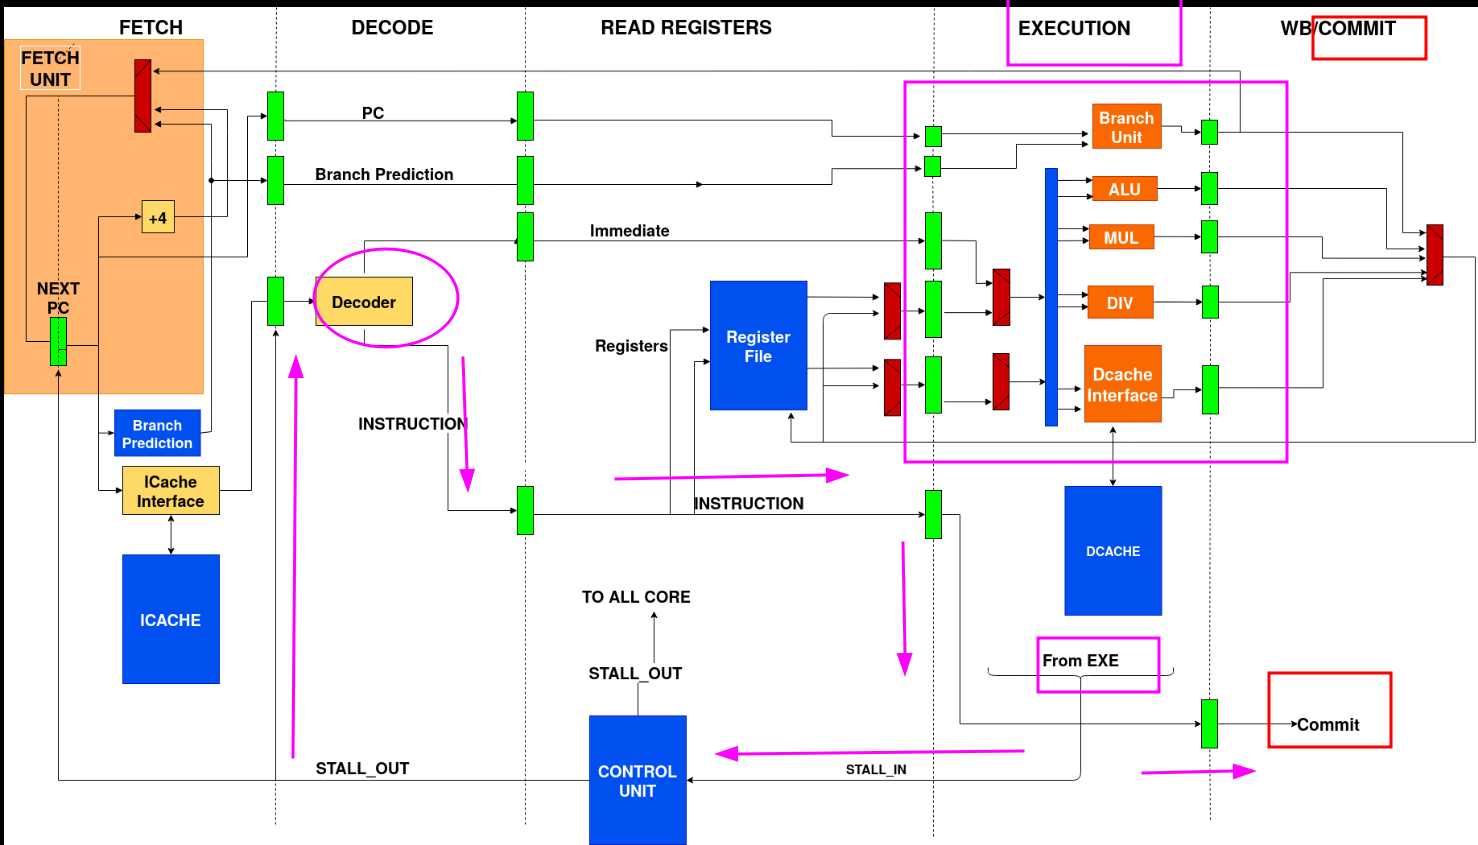
\includegraphics[width=\textwidth]{ch12_commit_overview.png}
  \caption{Commit stage in context, highlighting the decode-to-commit control path}
  \label{fig:commit-overview}
\end{figure}

\section{Reorder Buffer (ROB)}

Although the repository does not contain a standalone module named \rtl{rob.sv}, the
reorder/retirement functionality is implemented through the \textbf{Graduation List}, together with the
rename structures and control logic.

The Graduation List maintains the order of all in-flight instructions from dispatch until retirement.

For each instruction it tracks information such as:
\begin{itemize}
  \item destination physical register
  \item completion status
  \item exception status
  \item branch information
  \item retirement eligibility
\end{itemize}

When execution finishes, the corresponding entry is marked as completed. The Commit stage
continuously checks the oldest valid entry. If the instruction has completed without exceptions, it
is retired.

Thus, the Graduation List performs the architectural role traditionally associated with a Reorder
Buffer (ROB).

\begin{rtlrefs}
  \rtlitem{rtl/datapath/rtl/wb_stage/rtl/graduation_list.sv}
  \rtlitem{rtl/datapath/rtl/ir_stage/rtl/rename_table.sv}
  \rtlitem{rtl/datapath/rtl/ir_stage/rtl/free_list.sv}
\end{rtlrefs}

\begin{figure}[h]
  \centering
  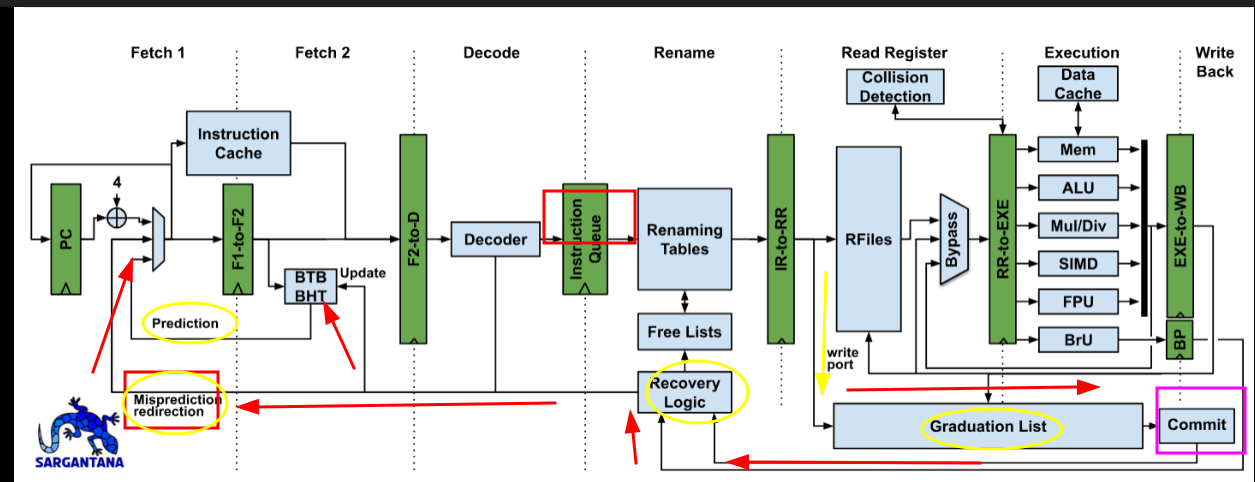
\includegraphics[width=\textwidth]{ch12_reorder_buffer.png}
  \caption{Graduation List acting as the Reorder Buffer: recovery and commit signal paths highlighted}
  \label{fig:reorder-buffer}
\end{figure}

\section{In-Order Retirement}

Although execution is highly parallel, retirement always occurs in program order.

For each instruction, the Commit stage performs several checks before retirement:
\begin{itemize}
  \item Has execution completed?
  \item Did the instruction raise an exception?
  \item Is it the oldest instruction?
  \item Are all previous instructions already retired?
\end{itemize}

Only after satisfying these conditions are the architectural structures updated.

Retirement includes:
\begin{itemize}
  \item updating the architectural register mapping
  \item releasing obsolete physical registers
  \item committing memory operations
  \item updating CSR state if required
  \item removing the instruction from the Graduation List
\end{itemize}

This mechanism ensures that software observes execution exactly as if instructions had been
executed sequentially.

\begin{rtlrefs}
  \rtlitem{rtl/datapath/rtl/wb_stage/rtl/graduation_list.sv}
  \rtlitem{rtl/datapath/rtl/ir_stage/rtl/free_list.sv}
  \rtlitem{rtl/datapath/rtl/ir_stage/rtl/rename_table.sv}
\end{rtlrefs}

\section{Exception Handling}

One of the primary responsibilities of the Commit stage is precise exception handling.

If an instruction reports an exception during execution, retirement stops when that instruction
reaches the head of the Graduation List.

The processor then:
\begin{itemize}
  \item flushes younger speculative instructions
  \item restores the correct architectural state
  \item redirects the PC to the exception handler
  \item updates the required CSRs
  \item resumes execution from the exception vector
\end{itemize}

Since no younger instruction has committed yet, software observes a perfectly precise
exception.

This behavior is one of the major advantages of separating execution from retirement.

\begin{rtlrefs}
  \rtlitem{rtl/control_unit/rtl/control_unit.sv}
  \rtlitem{rtl/datapath/rtl/wb_stage/rtl/graduation_list.sv}
  \rtlitem{rtl/datapath/interface_csr/rtl/csr_interface.sv}
\end{rtlrefs}

\section{Pipeline Flush and Recovery}

Whenever speculation proves incorrect, the Commit stage coordinates recovery.

Typical recovery events include:
\begin{itemize}
  \item Branch misprediction
  \item Exceptions
  \item Interrupts
  \item System reset
  \item CSR redirection
\end{itemize}

Recovery generally involves:
\begin{enumerate}
  \item stopping retirement,
  \item flushing younger instructions,
  \item restoring the correct rename state,
  \item recovering the free list,
  \item redirecting the Program Counter,
  \item restarting instruction fetch.
\end{enumerate}

Because retirement is always in-order, recovery restores the processor to a precise architectural
state.

\begin{rtlrefs}
  \rtlitem{rtl/control_unit/rtl/control_unit.sv}
  \rtlitem{rtl/datapath/rtl/if_stage_1/rtl/branch_predictor.sv}
  \rtlitem{rtl/datapath/rtl/if_stage_1/rtl/if_stage_1.sv}
  \rtlitem{rtl/datapath/rtl/wb_stage/rtl/graduation_list.sv}
  \rtlitem{rtl/datapath/rtl/ir_stage/rtl/rename_table.sv}
  \rtlitem{rtl/datapath/rtl/ir_stage/rtl/free_list.sv}
\end{rtlrefs}

\chapter{Recovery Mechanisms}

\section{Overview}

Recovery in DRAC ensures that the processor returns to a precise architectural state whenever
speculative execution fails or an exception occurs. Since the processor executes instructions
out-of-order, incorrect speculative instructions must be removed while preserving the committed
architectural state.

\section{Branch Misprediction Recovery}

This section covers:
\begin{itemize}
  \item Branch prediction in IF Stage 1
  \item Actual branch resolution in the Execution Stage (\rtl{branch\_unit.sv})
  \item Detection of incorrect prediction
  \item Redirecting the Program Counter
  \item Flushing younger speculative instructions
  \item Restoring rename mappings and scoreboard entries
\end{itemize}

\begin{rtlrefs}
  \rtlitem{rtl/datapath/rtl/if_stage_1/branch_predictor.sv}
  \rtlitem{rtl/datapath/rtl/if_stage_1/bimodal_predictor.sv}
  \rtlitem{rtl/datapath/rtl/if_stage_1/return_address_stack.sv}
  \rtlitem{rtl/datapath/rtl/exe_stage/branch_unit.sv}
  \rtlitem{rtl/datapath/rtl/ir_stage/rename_table.sv}
  \rtlitem{rtl/datapath/rtl/ir_stage/free_list.sv}
  \rtlitem{rtl/datapath/rtl/exe_stage/score_board_scalar.sv}
  \rtlitem{rtl/datapath/rtl/exe_stage/score_board_simd.sv}
  \rtlitem{rtl/control_unit/rtl/control_unit.sv}
\end{rtlrefs}

\section{Exception Recovery}

This section covers:
\begin{itemize}
  \item Arithmetic exceptions
  \item Illegal instructions
  \item Memory exceptions
  \item CSR exceptions
  \item Exception propagation
  \item Precise exception model
\end{itemize}

\begin{rtlrefs}
  \rtlitem{rtl/csr/}
  \rtlitem{rtl/datapath/rtl/interface_csr/csr_interface.sv}
  \rtlitem{rtl/control_unit/}
\end{rtlrefs}

\section{Pipeline Flush Mechanism}

This section covers:
\begin{itemize}
  \item Flush signal generation
  \item Invalidating pipeline entries
  \item Clearing issue queues
  \item Clearing scoreboards
  \item Clearing pending memory requests
  \item Cancelling speculative instructions
\end{itemize}

\begin{rtlrefs}
  \rtlitem{rtl/control_unit/}
  \rtlitem{rtl/datapath/rtl/exe_stage/rtl/pending_mem_req_queue.sv}
  \rtlitem{rtl/datapath/rtl/exe_stage/rtl/pending_fp_ops_queue.sv}
  \rtlitem{rtl/datapath/rtl/exe_stage/rtl/pending_vfp_ops_queue.sv}
  \rtlitem{rtl/datapath/rtl/exe_stage/rtl/load_store_queue.sv}
  \rtlitem{rtl/datapath/rtl/exe_stage/rtl/score_board_scalar.sv}
  \rtlitem{rtl/datapath/rtl/exe_stage/rtl/score_board_simd.sv}
\end{rtlrefs}

\section{Restarting Instruction Execution}

This section covers:
\begin{itemize}
  \item Redirect PC
  \item Restore rename state
  \item Resume fetch
  \item Continue normal execution
\end{itemize}

\begin{rtlrefs}
  \rtlitem{rtl/datapath/rtl/if_stage_1/}
  \rtlitem{rtl/datapath/rtl/ir_stage/}
  \rtlitem{rtl/control_unit/}
\end{rtlrefs}


\appendix
\chapter{CRUX of RTL Files and Status}

\begingroup
\renewcommand{\arraystretch}{1.3}
\begin{longtable}{@{}p{0.22\textwidth}p{0.5\textwidth}p{0.22\textwidth}@{}}
\toprule
\textbf{Chapter} & \textbf{RTL Modules / Files} & \textbf{Status} \\
\midrule
\endhead

Chapter 9. Execution Stage &
\rtl{exe\_stage.sv}, \rtl{alu.sv}, \rtl{alu\_add.sv}, \rtl{alu\_logic.sv}, \rtl{alu\_shift.sv}, \rtl{alu\_cmp.sv}, \rtl{branch\_unit.sv}, \rtl{mul\_unit.sv}, \rtl{div\_unit.sv}, \rtl{mem\_unit.sv}, \rtl{vagu.sv}, \rtl{load\_store\_queue.sv}, \rtl{store\_buffer.sv}, \rtl{score\_board\_scalar.sv}, \rtl{score\_board\_simd.sv}, \rtl{pending\_mem\_req\_queue.sv}, \rtl{pending\_fp\_ops\_queue.sv}
& \ding{51}\ Fully supported \\
\addlinespace

Chapter 10. Memory Subsystem &
\rtl{mem\_unit.sv}, \rtl{vagu.sv}, \rtl{load\_store\_queue.sv}, \rtl{store\_buffer.sv}, \rtl{pending\_mem\_req\_queue.sv}
& \ding{51}\ Mostly supported \\
\addlinespace

Chapter 11. Writeback Stage &
\rtl{wb\_stage/rtl/graduation\_list.sv}, completion signals coming from execution units
& $\triangle$ Partially supported \\
\addlinespace

Chapter 12. Commit Stage &
\rtl{wb\_stage/rtl/graduation\_list.sv}, \rtl{ir\_stage/rtl/rename\_table.sv}, \rtl{free\_list.sv}, scoreboard modules
& $\triangle$ Commit logic exists but there is no standalone ROB module \\
\addlinespace

Chapter 13. Recovery Mechanisms &
\rtl{branch\_unit.sv}, \rtl{branch\_predictor.sv}, \rtl{return\_address\_stack.sv}, \rtl{control\_unit.sv}, rename/free-list recovery logic
& $\triangle$ Supported through distributed logic rather than one recovery module \\

\bottomrule
\end{longtable}
\endgroup

\vspace{1cm}

\noindent\textbf{Legend:}
\begin{itemize}[leftmargin=*]
  \item[\ding{51}] Complete RTL coverage located and matched to the documentation.
  \item[$\triangle$] Functionality exists but is distributed across several modules rather than a single dedicated file.
\end{itemize}

% ============================================================
\chapter{Abbreviations and Acronyms}

\begingroup
\renewcommand{\arraystretch}{1.2}
\begin{longtable}{@{}p{0.15\textwidth}p{0.27\textwidth}p{0.50\textwidth}@{}}
\toprule
\textbf{Abbr.} & \textbf{Full Form} & \textbf{Description} \\
\midrule
\endhead
ALU & Arithmetic Logic Unit & Executes integer arithmetic and logical operations. \\
AGU & Address Generation Unit & Computes effective addresses for memory instructions. \\
BTB & Branch Target Buffer & Stores predicted branch target addresses. \\
BHT & Branch History Table & Stores branch prediction history. \\
CSR & Control and Status Register & Special-purpose processor registers used for control and exception handling. \\
CFI & Control-Flow Integrity & Security mechanism preventing illegal control-flow transfers. \\
CPI & Cycles Per Instruction & Average execution cycles required per instruction. \\
EX & Execute Stage & Pipeline stage where arithmetic, logical, and branch operations are executed. \\
FP & Floating Point & Arithmetic performed on floating-point numbers. \\
FPU & Floating Point Unit & Dedicated execution unit for floating-point instructions. \\
FSM & Finite State Machine & Hardware state machine controlling logic behavior. \\
GHR & Global History Register & Stores global branch history for branch prediction. \\
IF & Instruction Fetch & Pipeline stage responsible for fetching instructions. \\
ID & Instruction Decode & Pipeline stage where instructions are decoded. \\
IQ & Instruction Queue & Buffer storing renamed instructions awaiting execution. \\
IR & Instruction Rename & Pipeline stage performing register renaming. \\
ISA & Instruction Set Architecture & Software-visible processor architecture. \\
LSQ & Load Store Queue & Tracks pending memory operations while preserving memory ordering. \\
LPAD & Landing Pad Instruction & Zicfilp instruction used to validate indirect branch targets. \\
MEM & Memory Stage & Pipeline stage responsible for memory accesses. \\
OoO & Out-of-Order & Execution model allowing instructions to execute before older instructions when dependencies permit. \\
PC & Program Counter & Address of the current instruction. \\
PE & Processing Element & Basic computational element, typically used in vector or matrix accelerators. \\
RAT & Register Alias Table & Maps architectural registers to physical registers during renaming. \\
ROB & Reorder Buffer & Tracks in-flight instructions and commits them in program order. \\
RR & Register Read & Pipeline stage where source operands are read. \\
RTL & Register Transfer Level & Hardware description abstraction used in Verilog/SystemVerilog. \\
RAS & Return Address Stack & Hardware stack predicting return instruction targets. \\
SIMD & Single Instruction Multiple Data & Parallel execution model processing multiple data elements simultaneously. \\
SQ & Store Queue & Queue buffering store operations before retirement. \\
SS & Shadow Stack & Protected stack used by Zicfiss to validate return addresses. \\
SV & SystemVerilog & Hardware Description Language used for RTL implementation. \\
TB & Testbench & Verification environment for RTL simulation. \\
WB & Writeback & Pipeline stage where execution results are written back. \\
XLEN & Integer Register Width & Width of the architectural integer registers (e.g., 32-bit or 64-bit). \\
\bottomrule
\end{longtable}
\endgroup

% ============================================================
\chapter{Pipeline Stage Abbreviations}

\begin{center}
\renewcommand{\arraystretch}{1.3}
\begin{tabular}{@{}ll@{}}
\toprule
\textbf{Stage} & \textbf{Meaning} \\
\midrule
IF1 & Instruction Fetch Stage 1 \\
IF2 & Instruction Fetch Stage 2 \\
ID & Instruction Decode \\
IR & Instruction Rename \\
RR & Register Read \\
EX & Execute \\
MEM & Memory Access \\
WB & Writeback \\
Commit & Instruction Retirement / Graduation \\
\bottomrule
\end{tabular}
\end{center}

% ============================================================
\chapter{RTL Module Abbreviations}

\begingroup
\renewcommand{\arraystretch}{1.2}
\begin{longtable}{@{}p{0.35\textwidth}p{0.55\textwidth}@{}}
\toprule
\textbf{Module} & \textbf{Description} \\
\midrule
\endhead
\rtl{datapath.sv} & Top-level datapath implementation \\
\rtl{control\_unit.sv} & Processor control logic \\
\rtl{if\_stage\_1.sv} & First instruction fetch stage \\
\rtl{if\_stage\_2.sv} & Second instruction fetch stage \\
\rtl{decoder.sv} & Instruction decoder \\
\rtl{immediate.sv} & Immediate value generator \\
\rtl{rename\_table.sv} & Register alias table \\
\rtl{free\_list.sv} & Physical register allocator \\
\rtl{instruction\_queue.sv} & Issue queue \\
\rtl{regfile.sv} & Physical register file \\
\rtl{exe\_stage.sv} & Top-level execution stage \\
\rtl{branch\_unit.sv} & Branch execution logic \\
\rtl{alu.sv} & Arithmetic Logic Unit \\
\rtl{div\_unit.sv} & Integer divider \\
\rtl{mul\_unit.sv} & Integer multiplier \\
\rtl{mem\_unit.sv} & Memory execution unit \\
\rtl{load\_store\_queue.sv} & Load/Store Queue \\
\rtl{pending\_mem\_req\_queue.sv} & Pending memory request tracker \\
\rtl{pending\_fp\_ops\_queue.sv} & Pending floating-point operations \\
\rtl{score\_board\_scalar.sv} & Scalar dependency scoreboard \\
\rtl{score\_board\_simd.sv} & SIMD dependency scoreboard \\
\rtl{graduation\_list.sv} & Instruction commit list \\
\rtl{csr\_interface.sv} & CSR interface logic \\
\bottomrule
\end{longtable}
\endgroup

% ============================================================
\chapter{RISC-V Extensions Referenced}

\begin{center}
\renewcommand{\arraystretch}{1.3}
\begin{tabular}{@{}ll@{}}
\toprule
\textbf{Extension} & \textbf{Description} \\
\midrule
RV64 & 64-bit RISC-V base ISA \\
M & Integer Multiply/Divide Extension \\
A & Atomic Extension \\
F & Single-Precision Floating Point \\
D & Double-Precision Floating Point \\
C & Compressed Instructions \\
V & Vector Extension \\
Zfa & Additional Floating-Point Instructions \\
Zfh & Half-Precision Floating Point \\
Zvfhmin & Minimal Half-Precision Vector Extension \\
Zicfilp & Control-Flow Integrity Landing Pad Extension \\
Zicfiss & Control-Flow Integrity Shadow Stack Extension \\
\bottomrule
\end{tabular}
\end{center}

% ============================================================
\chapter{Execution Unit Components}

\begin{center}
\renewcommand{\arraystretch}{1.3}
\begin{tabular}{@{}ll@{}}
\toprule
\textbf{Component} & \textbf{Function} \\
\midrule
ALU & Integer arithmetic and logic \\
Branch Unit & Branch comparison and target computation \\
Divider & Integer division operations \\
Multiplier & Integer multiplication operations \\
Memory Unit & Load and store execution \\
SIMD Unit & Vector arithmetic execution \\
FPU & Floating-point execution \\
AGU & Effective address generation \\
Scoreboard & Dependency tracking \\
Pending Queues & Track unfinished operations \\
\bottomrule
\end{tabular}
\end{center}


\end{document}
